\chapter{KONTRIBUSI}
\sloppy

\section{Perancangan Arsitektur}

Perancangan arsitektur sistem merupakan tahap awal yang sangat penting dalam pengembangan perangkat lunak. Sebagai seorang \emph{software architect}, perancangan arsitektur yang baik memastikan bahwa sistem dapat memenuhi kebutuhan fungsional dan non-fungsional, serta mendukung kemudahan pengelolaan, keamanan, dan skalabilitas. 

\subsection{Identifikasi Kebutuhan Pengguna}
Tahap pertama dalam perancangan ini adalah melakukan identifikasi kebutuhan pengguna. Proses ini bertujuan untuk menentukan spesifikasi sistem secara terperinci, sehingga setiap kebutuhan pengguna dapat terakomodasi dalam desain sistem.

\subsection{Pemilihan Teknologi}
Pemilihan teknologi merupakan aspek kritis dalam desain arsitektur. Teknologi yang dipilih bertujuan untuk mendukung implementasi sistem yang efisien, handal, dan mudah dikembangkan di masa depan. Keputusan ini didasarkan pada tren teknologi terkini dan prinsip-prinsip desain perangkat lunak modern.

\subsection{Perancangan Arsitektur Aplikasi}
Perancangan arsitektur aplikasi dilakukan dengan mempertimbangkan kebutuhan pengguna dan teknologi yang dipilih. Arsitektur ini mencakup struktur frontend, backend, dan DevOps, yang dirancang untuk mendukung pengembangan sistem yang efisien, aman, dan mudah dikelola.

\section{Perancangan Teknologi yang Digunakan}
Teknologi yang digunakan dalam pengembangan sistem ini dipilih berdasarkan kebutuhan untuk efisiensi, keamanan, dan skalabilitas. Perancangan ini mencakup aspek general, frontend, backend, dan DevOps, yang dijelaskan secara terperinci berikut ini.

\subsection{General}
Untuk menjaga konsistensi dan efisiensi dalam pengembangan, sejumlah standar diterapkan. Penggunaan \emph{ESLint} dan \emph{Prettier} memastikan format kode yang konsisten di seluruh proyek, sehingga meminimalkan potensi kesalahan dan mempermudah kolaborasi antar pengembang. Selain itu, integrasi \emph{Husky} dengan \emph{pre-commit hooks} memastikan bahwa linting dan pemformatan dilakukan sebelum perubahan kode dikirim ke repositori. Langkah ini merupakan bagian dari kontrol kualitas sejak tahap awal pengembangan.

Pipeline \emph{CI/CD} yang diimplementasikan menggunakan \emph{GitHub Actions} mendukung proses pengembangan berkelanjutan. Pipeline ini mencakup linting, pengujian, dan \emph{build} otomatis, yang memberikan umpan balik cepat atas setiap perubahan kode. Selain itu, \emph{starter kit} yang mencakup konfigurasi linting, pipeline \emph{CI/CD}, dan struktur proyek yang terorganisir disediakan untuk memastikan pengembang dapat memulai proyek dengan standar yang seragam.

\subsection{Arsitektur Frontend}
\emph{Frontend} sistem ini dibangun menggunakan \emph{Next.js} sebagai kerangka kerja utama. \emph{Next.js} dipilih karena mendukung \emph{server-side rendering (SSR)} dan \emph{static site generation (SSG)}, yang meningkatkan waktu muat halaman serta memberikan pengalaman pengguna yang lebih baik. Untuk antarmuka pengguna, kombinasi \emph{Shadcn/UI} dan \emph{Tailwind CSS} digunakan, memungkinkan desain antarmuka yang responsif, konsisten, dan efisien. Selain itu, \emph{Framer Motion} diterapkan untuk menambahkan animasi dinamis dan transisi halaman, yang membuat pengalaman pengguna lebih menarik dan interaktif. 

Berdasarkan penjelasan diatas dibuat \emph{starter kit} yang mencakup konfigurasi \emph{Next.js}, integrasi \emph{Shadcn/UI} dan \emph{Tailwind CSS}, serta \emph{Framer Motion}. \emph{Starter kit} ini juga dilengkapi dengan \emph{CI/CD} yang telah dijelaskan pada subab general untuk mendukung pengembangan berkelanjutan. \emph{Starter kit} ini memastikan pengembangan \emph{frontend} yang konsisten dan efisien, serta mempercepat proses pengembangan antarmuka pengguna.

\subsection{Arsitektur Backend}
Di sisi \emph{backend}, \emph{AdonisJS v6} digunakan sebagai kerangka kerja utama. \emph{AdonisJS} dipilih karena mendukung pengembangan berbasis \emph{TypeScript} yang modular dan terorganisir. Untuk memastikan keamanan, sistem otentikasi dirancang menggunakan \emph{JWT (JSON Web Token)}, sehingga hanya pengguna yang terotorisasi dapat mengakses data sensitif. Dalam pengelolaan data, \emph{Lucid ORM} digunakan untuk mempermudah manipulasi database relasional, dengan \emph{PostgreSQL} sebagai database utama karena keandalannya dalam menangani data terstruktur. Selain itu, \emph{Redis} diintegrasikan sebagai \emph{caching layer} untuk meningkatkan kinerja aplikasi, terutama dalam pengelolaan sesi dan antrian pekerjaan. 

Berdasarkan penjelasan di atas, dibuat \emph{starter kit backend} yang mencakup struktur proyek \emph{AdonisJS}, integrasi \emph{Redis}, dan pipeline \emph{CI/CD}. \emph{Starter kit} ini juga mengimplementasikan pengujian otomatis (\emph{automated testing}) untuk memverifikasi integritas aplikasi setelah setiap pembaruan. Dengan demikian, pengembangan \emph{backend} menjadi lebih andal, konsisten, dan terukur.

\subsection{DevOps}
Pendekatan \emph{DevOps} yang digunakan mendukung pengelolaan sistem yang efisien dan terukur. \emph{Docker} digunakan untuk mengisolasi layanan \emph{frontend} dan \emph{backend}, memastikan konsistensi lingkungan di berbagai tahap pengembangan. Selain itu, \emph{docker-compose.yml} dirancang untuk mengelola layanan seperti \emph{backend}, \emph{PostgreSQL}, \emph{Redis}, dan \emph{Adminer}, sehingga integrasi layanan menjadi lebih mudah.

Untuk orkestrasi layanan, \emph{Kubernetes} digunakan. Konfigurasi mencakup \emph{namespace} untuk setiap layanan, \emph{deployment} yang mendukung skalabilitas, serta \emph{load balancer} untuk mengatur lalu lintas jaringan. \emph{Nginx} diterapkan sebagai \emph{reverse proxy} untuk mengelola permintaan ke sistem, memastikan pengelolaan lalu lintas yang efisien dan terstruktur.

\emph{Starter kit DevOps} mencakup template \emph{Dockerfile}, \emph{docker-compose.yml}, konfigurasi \emph{Nginx}, serta \emph{YAML Kubernetes} untuk \emph{deployment}. Kit ini juga mendukung pengelolaan log terpusat menggunakan \emph{ELK Stack (Elasticsearch, Logstash, dan Kibana)} untuk memantau performa dan memastikan sistem berjalan optimal. Dengan pendekatan ini, sistem dapat dikelola dengan standar yang tinggi, baik di lingkungan pengembangan maupun produksi.

\section{Arsitektur Aplikasi}
Arsitektur aplikasi PraktikaApp dirancang dengan pendekatan \emph{microservices} dan \emph{containerization} untuk mendukung modularitas, skalabilitas, dan kemudahan manajemen sistem. Pendekatan ini memungkinkan setiap layanan utama dapat dikembangkan, dikelola, dan diterapkan secara independen tanpa mengganggu layanan lainnya. Arsitektur ini terdiri dari tiga layanan utama, yaitu PraktikaApp, PraktikaTelelab, dan PraktikaSSO, yang masing-masing dipisahkan ke dalam kontainer terisolasi. PraktikaApp berfungsi sebagai sistem inti yang menangani administrasi praktikum, mencakup pengelolaan data mahasiswa, jadwal praktikum, pengaturan modul, dan pelaporan hasil. Layanan ini terdiri dari dua komponen utama, yaitu \emph{frontend} dan \emph{backend}, yang masing-masing diimplementasikan dalam kontainer terpisah untuk memastikan pengelolaan kode yang modular dan mempermudah skalabilitas.  
PraktikaTelelab dirancang untuk mendukung praktikum berbasis simulasi dan IoT, terutama untuk eksperimen rangkaian digital. Sistem ini terhubung dengan perangkat keras berbasis \emph{ESP} seperti \emph{ESP8266} atau \emph{ESP32}, yang memungkinkan pengguna untuk melakukan eksperimen jarak jauh. PraktikaTelelab tidak hanya menyediakan kemampuan simulasi berbasis perangkat lunak, tetapi juga memungkinkan integrasi langsung dengan perangkat keras fisik untuk memperkaya pengalaman praktikum. Hal ini memungkinkan mahasiswa untuk memahami implementasi praktis teknologi IoT secara langsung. Sementara itu, PraktikaSSO bertindak sebagai sistem \emph{Single Sign-On (SSO)} yang mengintegrasikan PraktikaApp, PraktikaTelelab, serta aplikasi lainnya yang akan dikembangkan di masa depan. PraktikaSSO memastikan bahwa pengguna dapat mengakses seluruh layanan dengan satu kredensial tunggal, sehingga meningkatkan efisiensi dan pengalaman pengguna secara keseluruhan. Sistem ini dirancang dengan keamanan yang tinggi untuk melindungi data sensitif dan mencegah akses tidak sah. Diagram arsitektur aplikasi secara keseluruhan dapat dilihat pada Gambar \ref{fig:app_architecture}.

\begin{figure}[H]
    \centering
    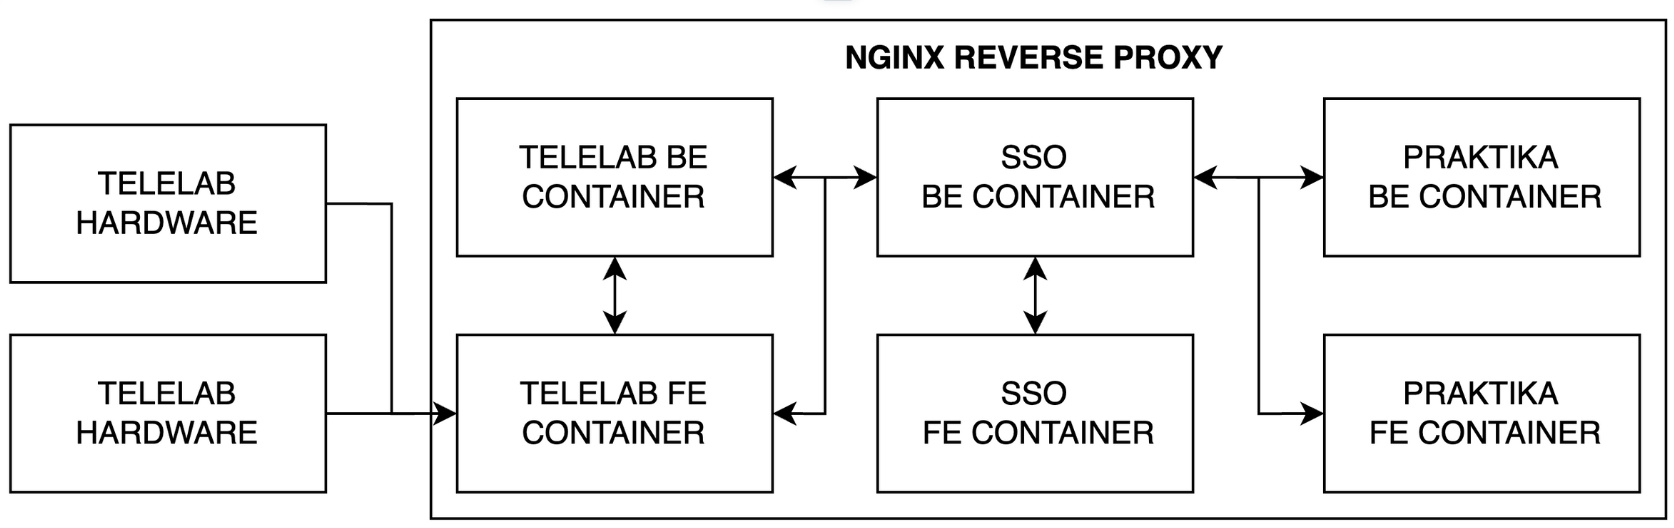
\includegraphics[width=0.8\textwidth]{gambar/app_architecture.png}
    \caption{Diagram Arsitektur Aplikasi}
    \label{fig:app_architecture}
\end{figure}

Untuk mendukung implementasi layanan-layanan tersebut, setiap kontainer dirancang dengan komponen-komponen utama yang saling melengkapi, seperti yang digambarkan pada Gambar \ref{fig:container_contents}. Kontainer \emph{Single BE Container} mencakup beberapa elemen penting, yaitu \emph{App Adminer}, sebuah alat antarmuka yang mempermudah pengelolaan database PostgreSQL melalui antarmuka web yang intuitif; \emph{App Postgres Database}, yang digunakan sebagai sistem manajemen basis data relasional untuk menyimpan data pengguna dan operasional aplikasi; \emph{App Backend}, yang bertanggung jawab untuk menjalankan logika bisnis aplikasi dan memproses permintaan dari \emph{frontend}; serta \emph{App Redis Session Storage}, yang digunakan untuk penyimpanan sesi berbasis memori guna meningkatkan performa dan manajemen sesi pengguna. Setiap komponen ini dirancang untuk bekerja secara terintegrasi, tetapi tetap terisolasi untuk memastikan keamanan dan stabilitas sistem.

\begin{figure}[H]
    \centering
    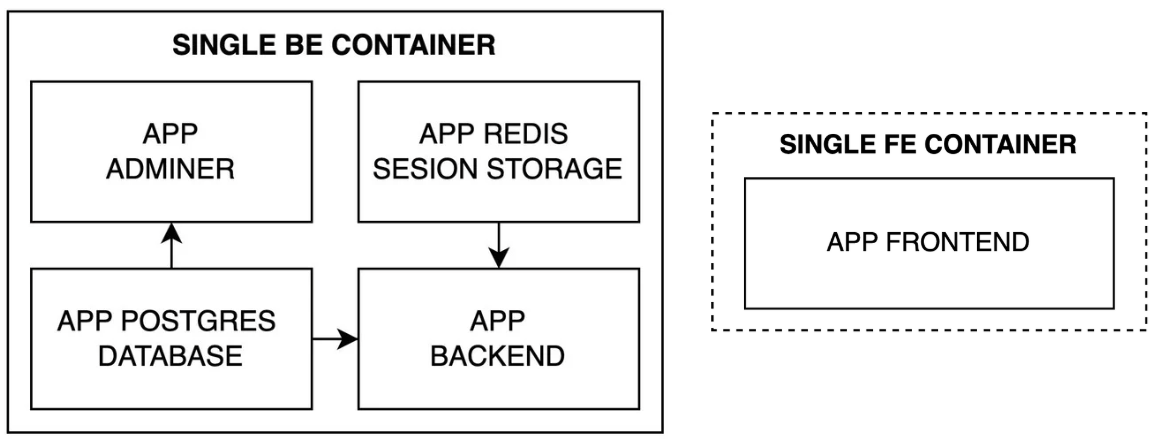
\includegraphics[width=0.6\textwidth]{gambar/container.png}
    \caption{Diagram Isi Kontainer}
    \label{fig:container_contents}
\end{figure}

Selain itu, kontainer \emph{Single FE Container} terdiri dari \emph{App Frontend}, yaitu antarmuka pengguna berbasis web yang berfungsi sebagai titik interaksi utama bagi pengguna aplikasi. Antarmuka ini dirancang dengan teknologi modern untuk memastikan pengalaman pengguna yang responsif, cepat, dan intuitif. Semua komunikasi antara \emph{frontend} dan \emph{backend} dikelola melalui protokol yang aman, memastikan integritas dan kerahasiaan data. Dengan pendekatan ini, arsitektur aplikasi PraktikaApp tidak hanya mendukung integrasi yang mudah antar layanan, tetapi juga memfasilitasi pengelolaan, pengujian, dan penerapan sistem di lingkungan pengembangan maupun produksi. Keunggulan ini memastikan bahwa aplikasi dapat terus berkembang seiring dengan kebutuhan pengguna dan perubahan teknologi tanpa mengorbankan stabilitas atau efisiensi.

\section{Pengembangan Backend}
Pengembangan \emph{backend} PraktikaApp dibatasi dalam dua langkah utama, yaitu pengembangan struktur kode dan pengujian fungsional. Pengembangan struktur kode dilakukan dengan memperhatikan prinsip-prinsip desain perangkat lunak yang baik, seperti modularitas, kohesi, dan dekapsulasi. Struktur kode yang baik memastikan bahwa sistem dapat dikembangkan, dikelola, dan diperbarui dengan mudah di masa depan. Selain itu, pengujian fungsional dilakukan untuk memverifikasi bahwa setiap fitur berjalan sesuai dengan spesifikasi yang ditentukan. Pengujian ini mencakup pengujian \emph{unit}, \emph{integration}, dan \emph{end-to-end} untuk memastikan bahwa setiap komponen berinteraksi dengan benar dan menghasilkan hasil yang diharapkan.

\subsection{Pengembangan Struktur Kode}
Struktur kode PraktikaApp dibatasi dalam dua bagian, yaitu \emph{API} dan \emph{Database}. Pengembangan \emph{API} dilakukan dengan memperhatikan prinsip \emph{RESTful API} yang baik, seperti penggunaan metode HTTP yang tepat, pengelolaan status kode yang konsisten, dan dokumentasi yang jelas. Struktur \emph{API} dirancang untuk mendukung operasi CRUD (Create, Read, Update, Delete) yang efisien, serta menyediakan antarmuka yang intuitif bagi pengguna. Selain itu, pengembangan \emph{database} dilakukan dengan memperhatikan desain basis data yang baik, seperti normalisasi, indeksasi, dan relasi yang tepat. Struktur \emph{database} dirancang untuk mendukung operasi pengelolaan data yang efisien, aman, dan terukur.

\subsection{Pengujian Fungsional}
Pengujian fungsional PraktikaApp dilakukan dengan menggunakan framework \emph{Jest} dan \emph{Supertest} yang memudahkan dalam pengujian \emph{unit} dan \emph{integration}. Pengujian ini mencakup pengujian operasi CRUD, autentikasi pengguna, otorisasi akses, serta pengelolaan sesi dan antrian pekerjaan. Setiap pengujian dirancang untuk memverifikasi bahwa setiap fitur berjalan sesuai dengan spesifikasi yang ditentukan, serta memberikan umpan balik yang jelas atas setiap perubahan kode. Dengan pendekatan ini, pengembangan \emph{backend} PraktikaApp menjadi lebih terstruktur, terukur, dan andal.

\section{Implementasi PraktikaSSO}
Implementasi PraktikaSSO memanfaatkan OpenID Connect dan OAuth 2.0 sebagai dasar untuk mengelola registrasi klien dan autentikasi pengguna secara aman. Sistem ini dirancang untuk memberikan pengalaman pengguna yang efisien dan nyaman, sekaligus memastikan keamanan data dan integritas sistem. Proses ini terdiri dari dua alur utama, yaitu registrasi klien dan autentikasi pengguna, yang masing-masing dijelaskan secara rinci berikut ini.

\subsection{Alur Registrasi Klien}
Registrasi klien merupakan langkah awal untuk mengintegrasikan aplikasi eksternal dengan PraktikaSSO. Proses ini diawali oleh pengembang aplikasi yang mengirimkan permintaan POST ke endpoint \texttt{/clients} di server OpenID dengan menyertakan kredensial pengembang. Server OpenID memvalidasi token pengembang untuk memastikan otentikasi dan otorisasi permintaan. Validasi ini penting untuk menjaga keamanan sistem dan mencegah akses tidak sah. Setelah token divalidasi, server OpenID menghasilkan \emph{client\_id} dan \emph{client\_secret} yang unik untuk setiap klien. Data ini disimpan dengan aman di basis data, memastikan bahwa setiap klien dapat dikenali dan dilacak dengan jelas. Akhirnya, server mengirimkan \emph{client\_id} dan \emph{client\_secret} kepada pengembang sebagai respons.  Diagram alur registrasi klien ditunjukkan pada Gambar \ref{fig:client_registration}.

\begin{figure}[H]
    \centering
    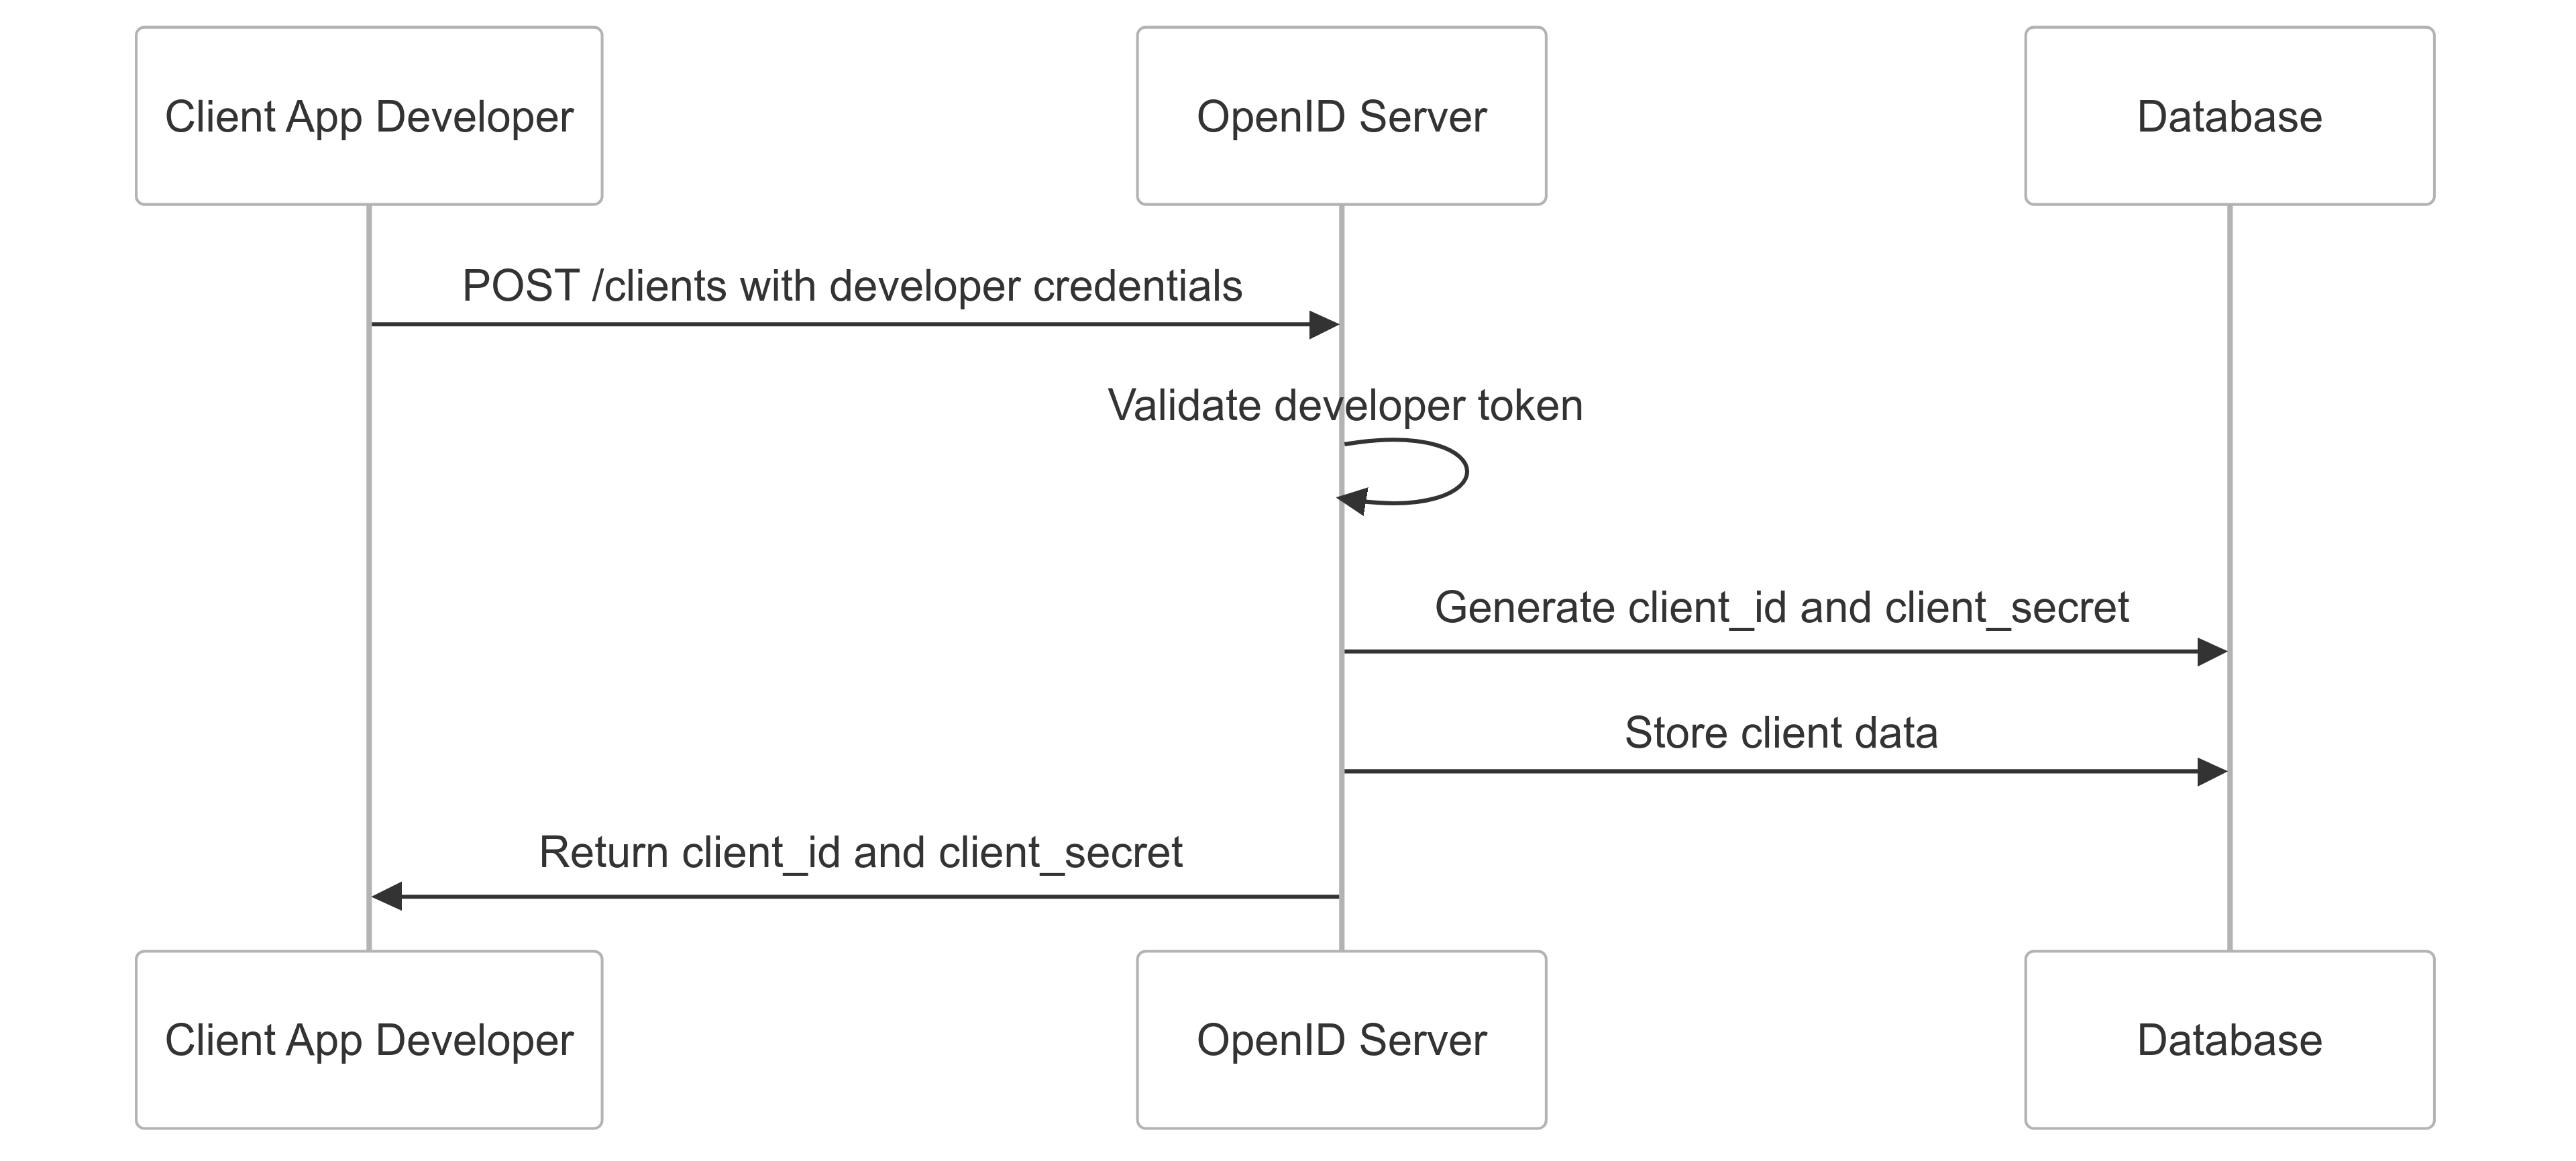
\includegraphics[width=0.9\textwidth]{gambar/create_client_flow.png}
    \caption{Diagram Alur Registrasi Klien}
    \label{fig:client_registration}
\end{figure}

\subsection{Alur Autentikasi Pengguna}
Setelah klien terdaftar, pengguna dapat mengakses aplikasi melalui alur autentikasi yang dirancang menggunakan protokol OpenID Connect dan OAuth 2.0. Alur ini bertujuan untuk memastikan bahwa hanya pengguna yang sah dapat mengakses sumber daya yang dilindungi. Proses autentikasi dimulai ketika pengguna menekan tombol login pada aplikasi klien. Pada tahap ini, aplikasi klien mengirimkan permintaan GET ke endpoint \texttt{/authorize} di server OpenID. Permintaan ini mencakup beberapa parameter penting, yaitu \emph{client\_id}, \emph{redirect\_uri}, \emph{response\_type=code}, \emph{scope}, \emph{state}, dan \emph{nonce}. Parameter \emph{client\_id} digunakan untuk mengidentifikasi aplikasi klien, sementara \emph{redirect\_uri} menentukan URL tempat pengguna akan diarahkan setelah proses autentikasi berhasil. Parameter \emph{response\_type=code} menunjukkan bahwa alur yang digunakan adalah Authorization Code Flow, yang merupakan salah satu alur OAuth 2.0 yang paling aman. Parameter \emph{scope} mendefinisikan tingkat akses yang diminta oleh aplikasi, seperti akses ke data pengguna. Sementara itu, \emph{state} dan \emph{nonce} digunakan untuk mencegah serangan replay dan memastikan integritas proses autentikasi.

Setelah permintaan diterima, server OpenID memvalidasi parameter \emph{client\_id} dan \emph{redirect\_uri} terhadap data yang tersimpan di basis data. Validasi ini penting untuk memastikan bahwa permintaan berasal dari aplikasi klien yang telah terdaftar dan disetujui. Jika validasi berhasil, server memeriksa apakah token pengguna yang sah sudah ada. Jika token tidak ditemukan atau telah kedaluwarsa, server meminta pengguna untuk melakukan autentikasi ulang dengan memasukkan kredensial mereka, seperti email dan kata sandi. Setelah pengguna berhasil diautentikasi, server OpenID menghasilkan \emph{auth\_code} (kode otorisasi) yang bersifat sementara. Kode ini disimpan di basis data untuk keperluan validasi lebih lanjut dan dikirimkan kembali ke aplikasi klien melalui \emph{redirect\_uri} yang telah ditentukan sebelumnya.

Pada tahap berikutnya, aplikasi klien mengirimkan permintaan POST ke endpoint \texttt{/token}. Permintaan ini mencakup \emph{auth\_code} yang diterima sebelumnya, bersama dengan \emph{client\_id} dan \emph{client\_secret}. Server OpenID memvalidasi \emph{auth\_code} untuk memastikan bahwa kode tersebut belum digunakan atau kedaluwarsa, serta memeriksa kredensial klien untuk memastikan bahwa permintaan berasal dari aplikasi yang sah. Setelah validasi berhasil, server menghasilkan \emph{access token} dan \emph{ID token}. \emph{Access token} digunakan oleh aplikasi klien untuk mengakses API yang dilindungi, sedangkan \emph{ID token} berisi informasi pengguna dalam format terstruktur yang memungkinkan aplikasi klien untuk mengidentifikasi pengguna tanpa memerlukan panggilan tambahan ke server.

Aplikasi klien kemudian dapat menggunakan \emph{access token} untuk mengakses sumber daya yang dilindungi, seperti data pengguna. Untuk mendapatkan informasi pengguna secara spesifik, aplikasi klien dapat mengirimkan permintaan GET ke endpoint \texttt{/userinfo}, dengan menyertakan \emph{access token} dalam header permintaan. Server OpenID memvalidasi \emph{access token} dan mengambil data pengguna dari basis data. Data ini kemudian dikembalikan ke aplikasi klien dalam format JSON yang dapat langsung digunakan untuk menampilkan informasi pengguna atau keperluan lainnya. Alur autentikasi ini dirancang untuk memastikan keamanan dan efisiensi, dengan memanfaatkan fitur enkripsi dalam proses pengiriman data sensitif. Penggunaan \emph{state} dan \emph{nonce} memberikan perlindungan tambahan terhadap serangan seperti \emph{Cross-Site Request Forgery (CSRF)} dan \emph{replay attacks}. Selain itu, validasi berlapis terhadap \emph{client\_id}, \emph{redirect\_uri}, dan \emph{auth\_code} memastikan bahwa hanya aplikasi dan pengguna yang sah yang dapat mengakses sistem. Diagram alur autentikasi pengguna ditampilkan pada Gambar \ref{fig:auth_flow}.

\begin{figure}[H]
    \centering
    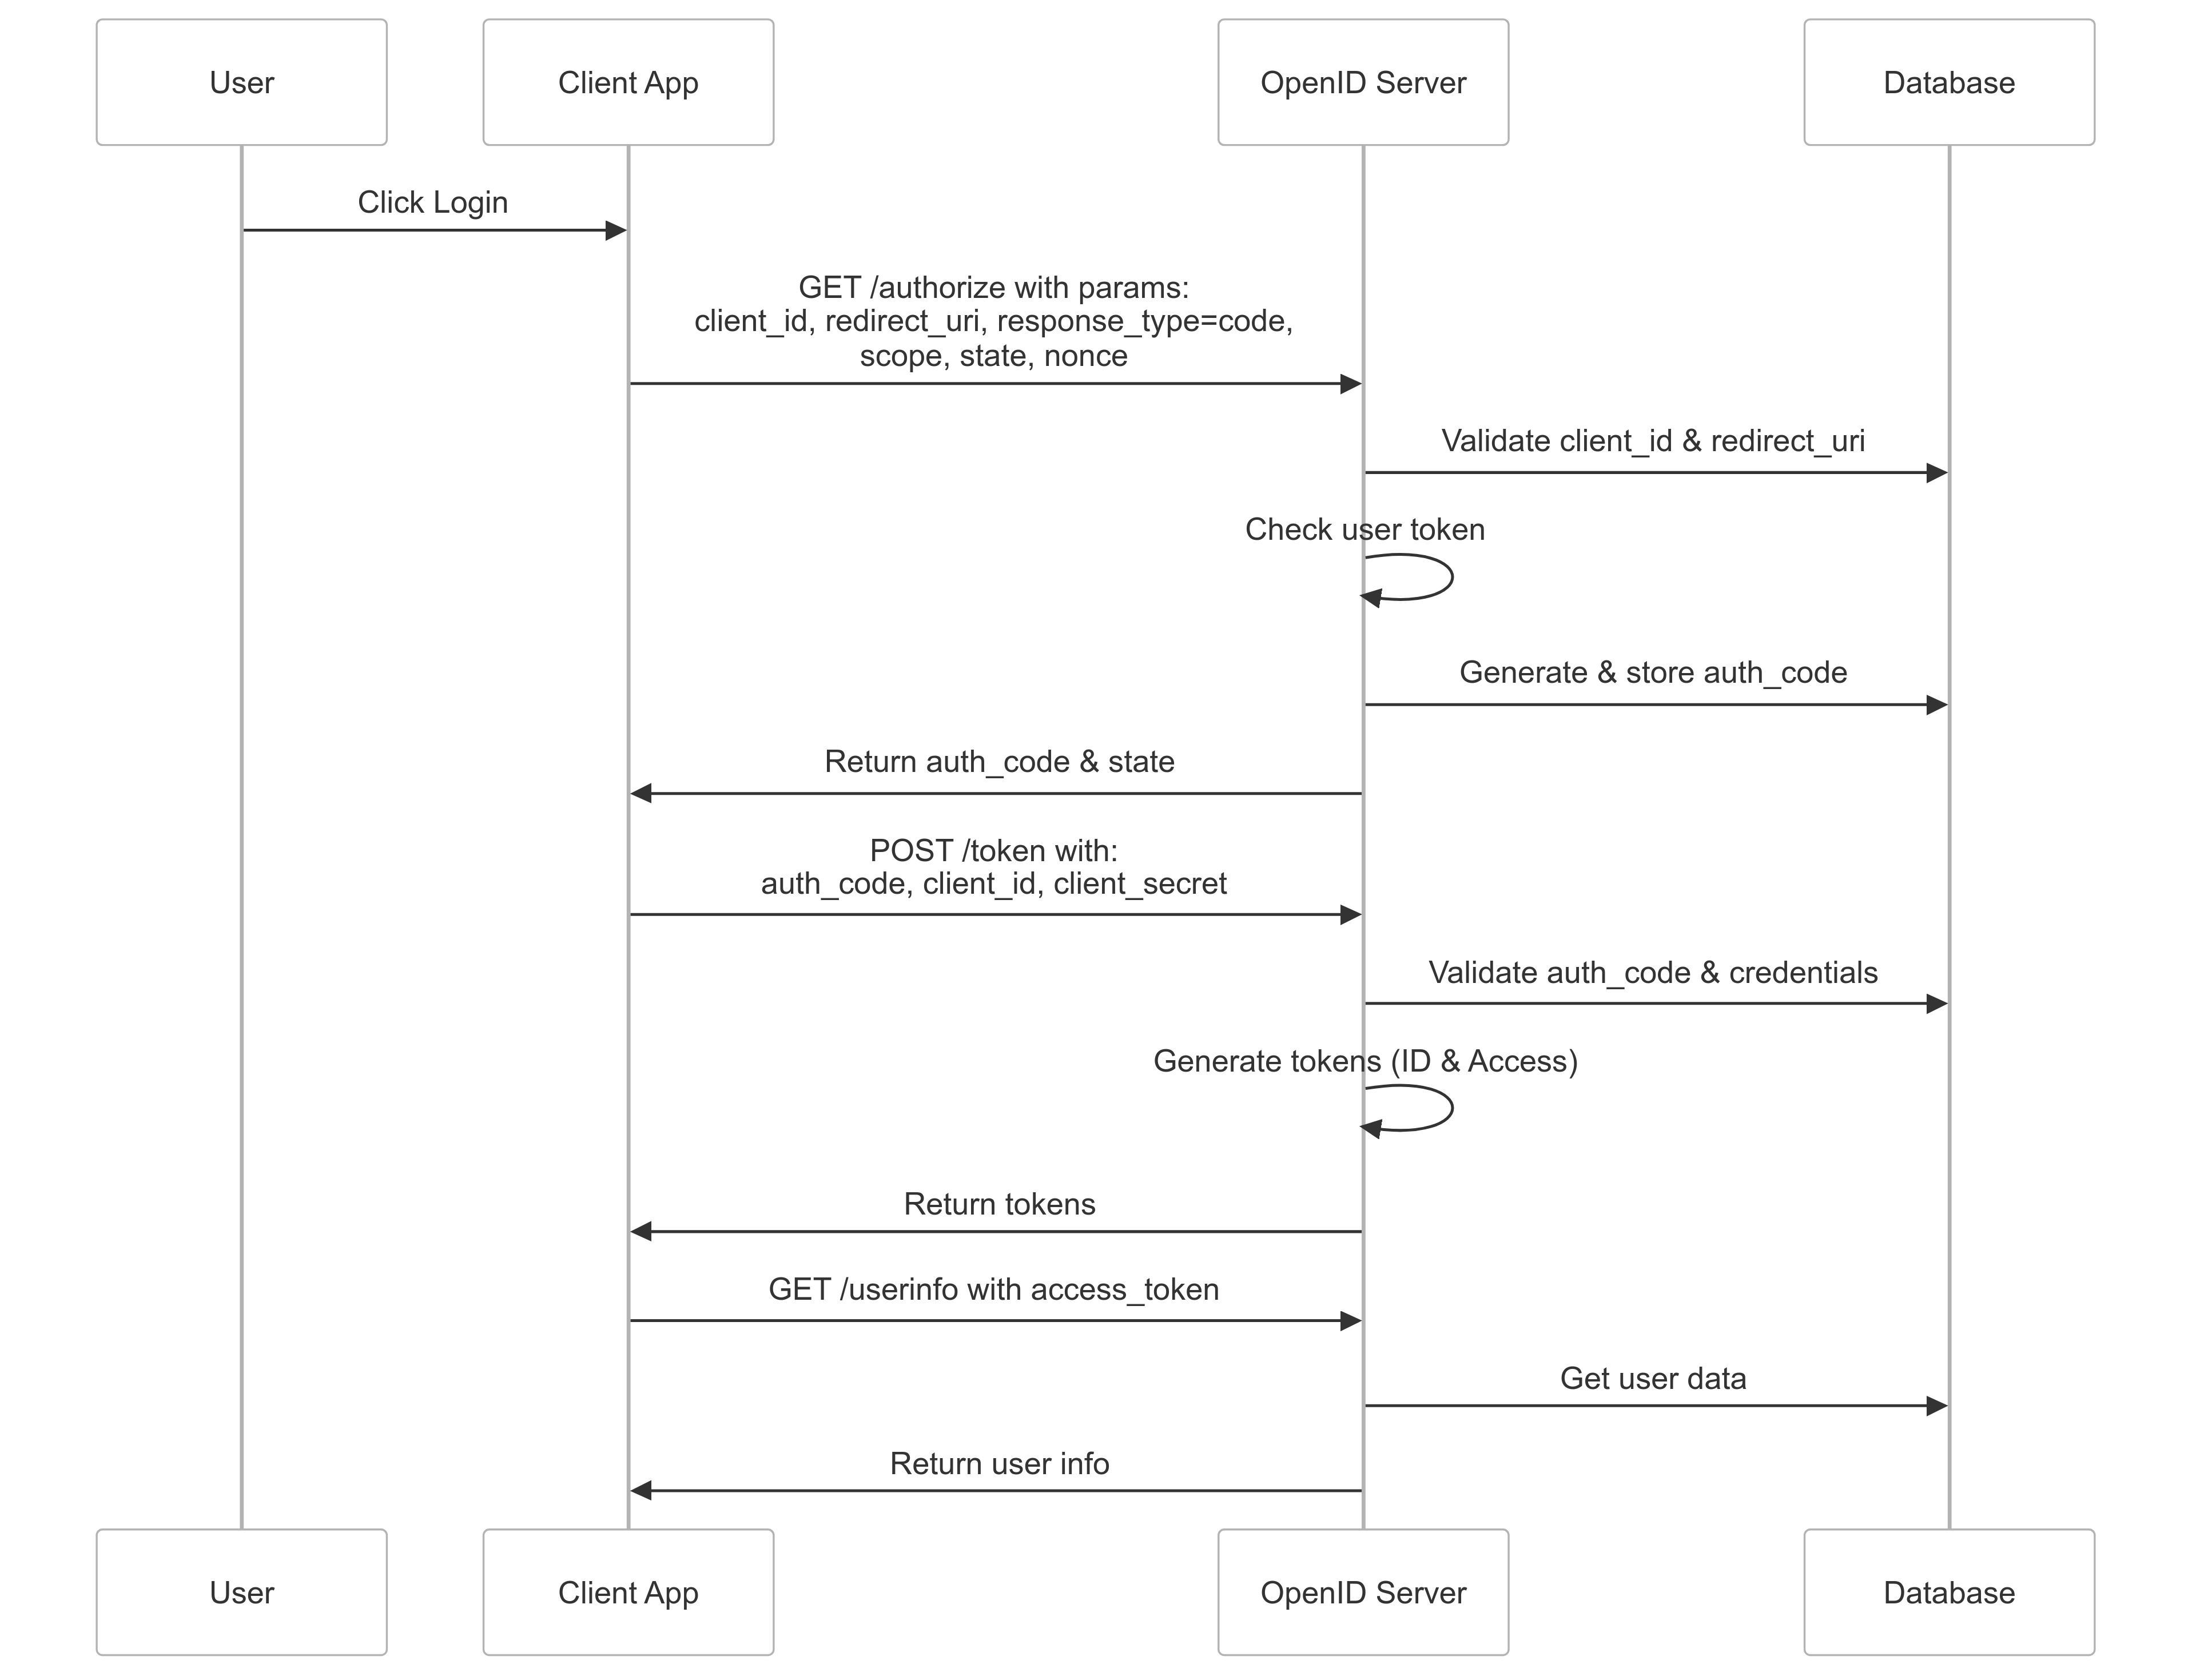
\includegraphics[width=1\textwidth]{gambar/auth_flow.png}
    \caption{Diagram Alur Autentikasi Pengguna}
    \label{fig:auth_flow}
\end{figure}


\subsection{Pemilihan OpenID Connect dan OAuth 2.0}
OpenID Connect dan OAuth 2.0 dipilih sebagai protokol dasar untuk PraktikaSSO karena beberapa alasan utama yang berkaitan dengan keamanan, fleksibilitas, dan skalabilitas. OpenID Connect adalah standar terbuka yang memungkinkan autentikasi berbasis web dengan cara yang sederhana namun aman. Dengan menggunakan OpenID Connect, PraktikaSSO dapat menyediakan mekanisme \emph{Single Sign-On (SSO)} yang memungkinkan pengguna mengakses berbagai aplikasi dengan satu kredensial tunggal. Hal ini tidak hanya meningkatkan pengalaman pengguna tetapi juga mengurangi risiko keamanan terkait dengan pengelolaan banyak akun dan kata sandi.

OAuth 2.0, sebagai protokol otorisasi, memberikan fleksibilitas untuk mengatur izin akses ke sumber daya tertentu tanpa mengungkapkan kredensial pengguna. Dengan mendukung alur seperti \emph{Authorization Code Flow}, OAuth 2.0 memungkinkan PraktikaSSO untuk mengelola otorisasi dengan aman di berbagai skenario, termasuk aplikasi berbasis web, seluler, dan layanan API.Kombinasi OpenID Connect dan OAuth 2.0 memberikan fondasi yang kuat untuk PraktikaSSO, memastikan bahwa autentikasi dan otorisasi dilakukan sesuai dengan standar industri. Selain itu, protokol ini memungkinkan PraktikaSSO untuk berkembang dan mendukung lebih banyak aplikasi serta integrasi di masa depan, tanpa mengorbankan keamanan atau efisiensi.


\section{Implementasi PraktikaApp Backend}
Implementasi PraktikaApp Backend merupakan realisasi dari desain arsitektur yang telah dijelaskan sebelumnya, dengan menggunakan \emph{AdonisJS v6} sebagai kerangka kerja utama. Sistem ini dikembangkan untuk mengelola seluruh aspek administrasi praktikum, mulai dari perencanaan hingga evaluasi, dengan memanfaatkan fitur modular dan keamanan berbasis \emph{JWT (JSON Web Token)}. Dengan pendekatan ini, PraktikaApp mampu mengintegrasikan berbagai peran pengguna dan alur kerja yang kompleks ke dalam satu sistem yang terorganisir. Pada tahap implementasi, struktur proyek yang dirancang dengan \emph{starter kit} memungkinkan pengembangan modul berbasis \emph{Domain-Driven Design (DDD)}. Modul ini mencakup fitur utama seperti pembuatan praktikum, penjadwalan, penilaian, dan pengelolaan pengguna. Integrasi dengan \emph{PostgreSQL} melalui \emph{Lucid ORM} memungkinkan pengelolaan data yang efisien, termasuk penyimpanan informasi praktikum, jadwal, modul, nilai, serta data pengguna. Selain itu, \emph{Redis} digunakan untuk meningkatkan kinerja melalui penyimpanan sesi berbasis memori dan pengelolaan antrian pekerjaan, yang sangat berguna dalam memproses permintaan pengguna secara paralel.

Alur implementasi PraktikaApp Backend dimulai dengan admin yang membuat praktikum dan menetapkan dosen pengampu sebagai pengelola utama. Proses ini mencerminkan fleksibilitas yang ditawarkan oleh kerangka kerja \emph{AdonisJS}, di mana modul \emph{CRUD} (Create, Read, Update, Delete) diterapkan untuk mengelola data praktikum secara dinamis. Setelah dosen pengampu membuka praktikum, sistem mengizinkan mereka untuk menetapkan koordinator praktikum yang bertanggung jawab untuk tugas-tugas operasional, seperti pembuatan jadwal, penambahan modul, dan pengaturan parameter penilaian.Selama pelaksanaan praktikum, asisten praktikum menggunakan modul \emph{backend} untuk mengelola sesi praktikum, termasuk membuka sesi, mencatat kehadiran, dan memberikan penilaian individu. Sistem ini didukung oleh pipeline \emph{CI/CD} yang mengotomatisasi pengujian dan penerapan kode, memastikan bahwa setiap pembaruan tidak mengganggu fungsionalitas yang ada. Diagram alur awal yang mencakup peran admin, dosen pengampu, koordinator praktikum, dan mahasiswa ditunjukkan pada Gambar \ref{fig:initial_flow}.

\begin{figure}[H]
    \centering
    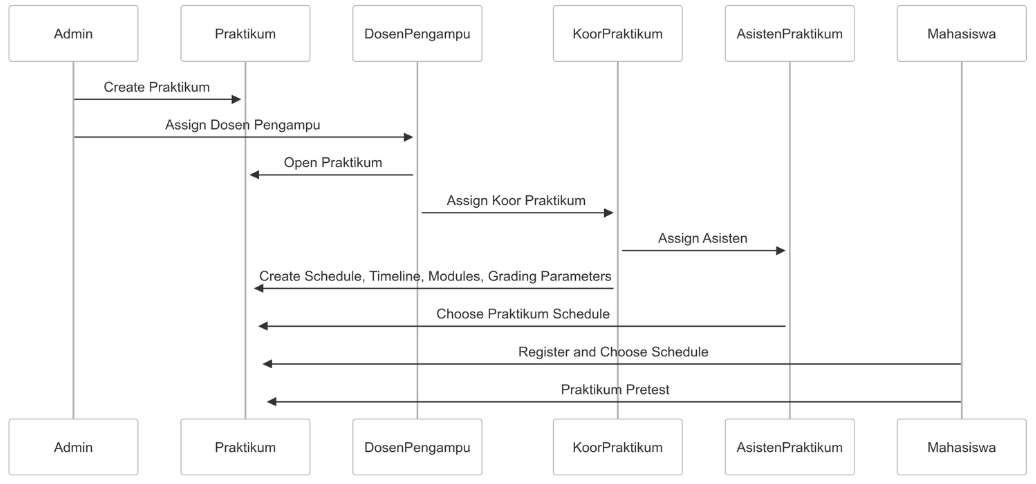
\includegraphics[width=0.9\textwidth]{gambar/init_flow.png}
    \caption{Diagram Alur Awal PraktikaApp}
    \label{fig:initial_flow}
\end{figure}

Sistem PraktikaApp Backend juga dirancang untuk menangani perubahan jadwal (reschedule). Fitur ini mengandalkan kekuatan \emph{AdonisJS} dalam memproses permintaan dinamis, di mana mahasiswa yang berhalangan hadir dapat mengajukan reschedule melalui sistem, yang kemudian akan diproses oleh asisten praktikum. Jadwal baru disimpan ke dalam \emph{PostgreSQL} dan diinformasikan kepada mahasiswa melalui pengumuman otomatis.

Diagram alur pelaksanaan praktikum, seperti yang ditampilkan pada Gambar \ref{fig:practicum_flow}, mencerminkan kemampuan sistem untuk mendukung interaksi yang berkelanjutan antara asisten praktikum dan mahasiswa. Setiap penilaian, baik untuk pelaksanaan praktikum maupun laporan sementara, disimpan dengan aman menggunakan mekanisme \emph{JWT}, memastikan bahwa hanya pengguna yang berwenang dapat mengakses data tersebut.

\begin{figure}[H]
    \centering
    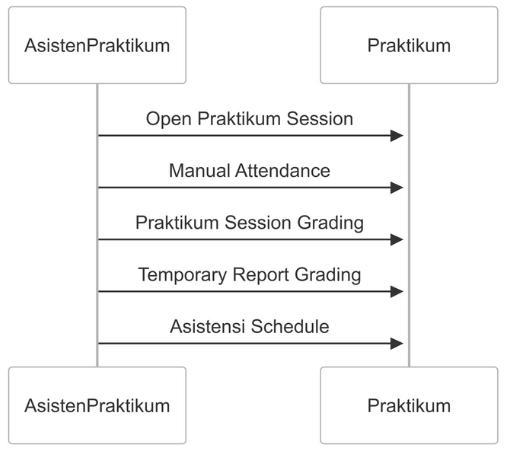
\includegraphics[width=0.5\textwidth]{gambar/prac_flow.png}
    \caption{Diagram Alur Pelaksanaan Praktikum}
    \label{fig:practicum_flow}
\end{figure}

Dalam proses penilaian akhir, koordinator praktikum memvalidasi semua nilai yang telah dimasukkan oleh asisten praktikum sebelum memberikan persetujuan. Setelah itu, dosen pengampu dapat melakukan tinjauan akhir dan mengesahkan nilai mahasiswa. Proses ini memanfaatkan pengelolaan data relasional di \emph{PostgreSQL} untuk memastikan bahwa semua data penilaian terdokumentasi dengan baik dan dapat diaudit. Sistem ini dirancang untuk mengelola berbagai peran pengguna dalam administrasi praktikum, dengan akses dan fungsi yang berbeda berdasarkan jenis pengguna, seperti yang ditunjukkan pada Gambar \ref{fig:user_roles}.

\begin{figure}[H]
    \centering
    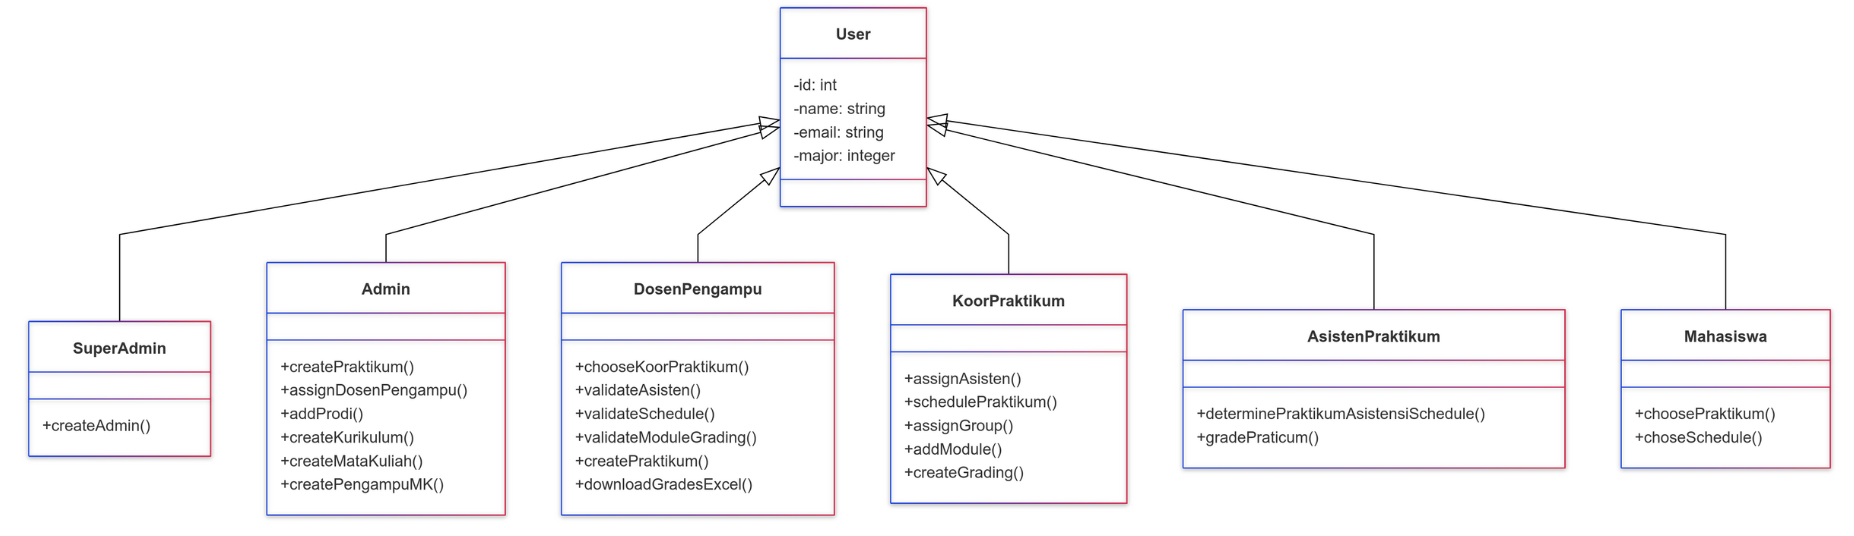
\includegraphics[width=1\textwidth]{gambar/class_diagram.png}
    \caption{Diagram Hak Akses Pengguna pada PraktikaApp}
    \label{fig:user_roles}
\end{figure}

Diagram pada Gambar \ref{fig:user_roles} menunjukkan bahwa PraktikaApp memiliki hierarki pengguna yang berbasis pada satu entitas utama, yaitu \emph{User}. Kelas \emph{User} memiliki atribut inti seperti \emph{id}, \emph{name}, \emph{email}, dan \emph{major}, yang dikelola di \emph{PostgreSQL} sebagai database utama. Berdasarkan atribut ini, pengguna dapat diberi peran yang lebih spesifik, termasuk \emph{SuperAdmin}, \emph{Admin}, \emph{DosenPengampu}, \emph{KoorPraktikum}, \emph{AsistenPraktikum}, dan \emph{Mahasiswa}. Setiap peran memiliki akses ke fungsi tertentu yang diimplementasikan dalam modul \emph{backend}. Sebagai contoh, \emph{SuperAdmin} memiliki hak penuh untuk membuat pengguna baru, termasuk \emph{Admin}, dan mengelola semua data dalam sistem. \emph{Admin} bertanggung jawab untuk membuat praktikum, menetapkan dosen pengampu, menambahkan program studi, serta membuat kurikulum dan mata kuliah. \emph{DosenPengampu} memiliki akses untuk memilih koordinator praktikum, memvalidasi jadwal, modul, dan penilaian, serta mengunduh nilai mahasiswa dalam format Excel. \emph{KoorPraktikum} bertugas untuk menetapkan asisten praktikum, menjadwalkan kegiatan praktikum, menambahkan modul, serta membuat parameter penilaian. \emph{AsistenPraktikum} bertanggung jawab untuk menentukan jadwal praktikum dan asistensi, serta memberikan penilaian terhadap pelaksanaan praktikum. Sementara itu, \emph{Mahasiswa} hanya dapat memilih praktikum dan jadwal yang sesuai dengan kebutuhan mereka.

Implementasi fungsi ini menggunakan \emph{AdonisJS}, yang menyediakan kemampuan modular untuk menangani logika bisnis secara terpisah berdasarkan peran pengguna. Sistem otentikasi menggunakan \emph{JWT (JSON Web Token) } dari Praktika SSO memastikan bahwa setiap pengguna hanya dapat mengakses fitur yang sesuai dengan perannya. Integrasi dengan \emph{Redis} digunakan untuk mempercepat proses otentikasi dan pengelolaan sesi pengguna. Melalui arsitektur ini, PraktikaApp Backend memberikan solusi yang terstruktur untuk mendukung berbagai alur kerja praktikum, mulai dari pembuatan hingga evaluasi. Setiap modul backend dirancang untuk mendukung komunikasi yang aman dan efisien antara klien dan server, memastikan bahwa data pengguna dan operasi sistem tetap terjaga integritasnya.

\section{Implementasi dan Alur Kerja Sistem PraktikaTelelab}
PraktikaTelelab merupakan platform yang dirancang untuk mendukung eksperimen praktikum berbasis simulasi dan IoT, dengan memanfaatkan teknologi modern seperti \emph{AdonisJS}, \emph{PostgreSQL}, dan \emph{Redis}. Sistem ini dirancang agar mahasiswa dapat menjalankan eksperimen secara fleksibel, baik secara daring melalui simulasi maupun luring dengan perangkat keras berbasis \emph{ESP32} yang terpasang pada modul praktikum rangkaian digital. Berikut adalah penjelasan mendalam mengenai alur kerja sistem serta implementasi di sisi \emph{backend}.

\subsection{Alur Kerja Sistem PraktikaTelelab}
Peserta yang telah terdaftar dalam praktikum rangkaian digital di PraktikaApp akan dapat mengakses PraktikaTelelab. PraktikaTelelab kemudian melakukan pengecekan terhadap jadwal dan jenis praktikum, baik yang dilakukan secara daring maupun luring, berdasarkan data yang terintegrasi dengan PraktikaApp. Setelah melakukan sinkronisasi data jadwal dengan PraktikaApp, peserta dapat memilih modul eksperimen yang ingin dijalankan, baik berupa simulasi daring maupun eksperimen luring. 

Jika peserta mendapatkan giliran praktikum dalam mode luring, PraktikaTelelab memanfaatkan perangkat keras berbasis IoT, seperti \emph{ESP32}, yang dipasang pada modul rangkaian digital. Mahasiswa menerima kredensial unik yang dihasilkan oleh backend, yang memungkinkan mereka mengakses modul eksperimen secara fisik. Kredensial ini disimpan sementara di \emph{Redis} untuk memastikan akses yang cepat dan aman. Mahasiswa kemudian dapat menjalankan eksperimen menggunakan perangkat keras, dan hasil eksperimen dikirim kembali ke sistem backend untuk diverifikasi. Backend memastikan bahwa hasil eksperimen luring memiliki integritas yang setara dengan eksperimen simulasi.Sementara itu, jika praktikum dilaksanakan dalam mode daring, mahasiswa dapat langsung mengakses modul simulasi praktikum melalui antarmuka yang disediakan oleh sistem. Setelah memilih modul eksperimen yang diinginkan, mahasiswa dapat memulai simulasi dan menguji eksperimen secara langsung. Sistem ini memungkinkan mahasiswa untuk melakukan uji coba sebanyak yang diperlukan sebelum menyerahkan hasil akhir. Setelah eksperimen selesai, hasil simulasi dikirim melalui sistem untuk diverifikasi dan divalidasi oleh asisten praktikum.

Diagram alur kerja sistem PraktikaTelelab dapat dilihat pada Gambar \ref{fig:telelab_flow}.

\begin{figure}[H]
\centering
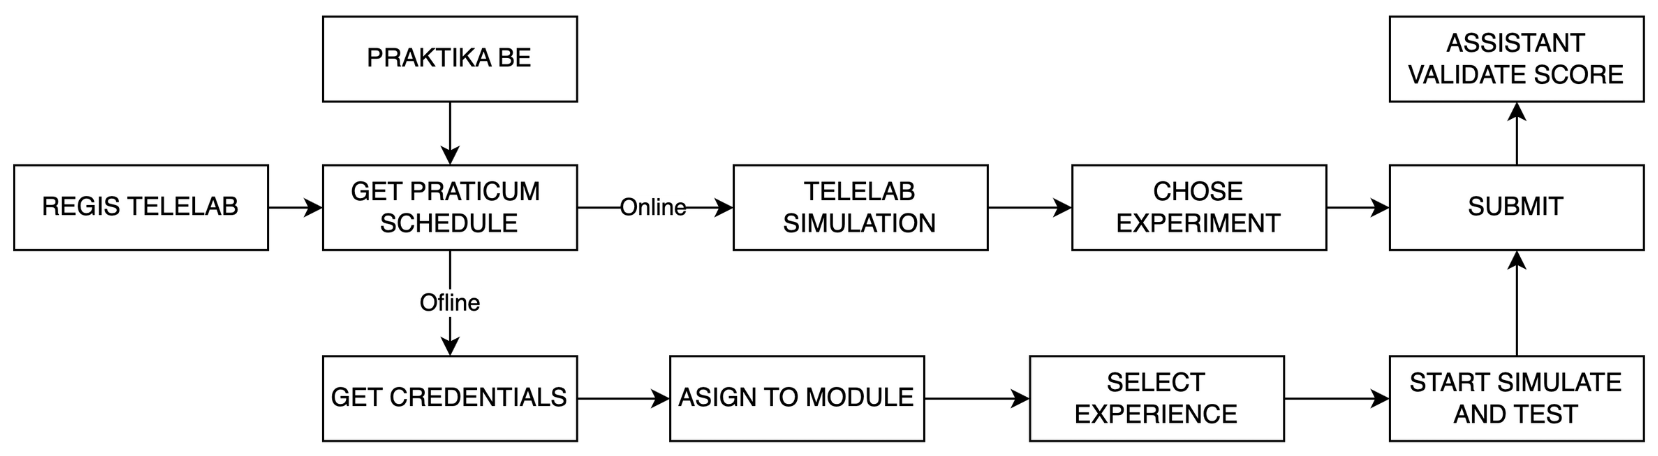
\includegraphics[width=0.9\textwidth]{gambar/telelab.png}
\caption{Diagram Alur Kerja Sistem PraktikaTelelab}
\label{fig:telelab_flow}
\end{figure}

\subsection{Implementasi Backend PraktikaTelelab}
Pada sisi \emph{backend}, PraktikaTelelab dirancang menggunakan kerangka kerja \emph{AdonisJS}, yang mendukung pengelolaan logika bisnis secara modular. Backend diimplementasikan dengan pendekatan \emph{Domain-Driven Design (DDD)}, yang memungkinkan setiap modul—seperti pendaftaran, pengelolaan jadwal, dan penilaian eksperimen—untuk dikelola secara independen namun tetap terintegrasi dalam satu sistem. 

Basis data relasional \emph{PostgreSQL} digunakan untuk menyimpan data utama, seperti informasi mahasiswa, jadwal praktikum, hasil eksperimen, dan penilaian. Dengan dukungan fitur-fitur seperti indeks, relasi antar tabel, dan transaksi, \emph{PostgreSQL} memastikan data disimpan dengan konsisten dan dapat diakses secara efisien.

Untuk meningkatkan performa, \emph{Redis} digunakan sebagai \emph{caching layer}. Teknologi ini mempermudah pengelolaan sesi pengguna, menyimpan kredensial sementara, dan mempercepat akses ke data yang sering digunakan selama proses simulasi. \emph{Redis} juga berperan penting dalam menjaga responsivitas sistem, meskipun ada banyak permintaan yang datang secara bersamaan.

\subsection{Validasi dan Penilaian Hasil Eksperimen}
Proses validasi dan penilaian hasil eksperimen sepenuhnya dilakukan di sisi \emph{backend}. Data hasil eksperimen, baik yang berasal dari simulasi maupun perangkat keras, akan diverifikasi untuk memastikan keaslian dan integritasnya sebelum diteruskan kepada asisten praktikum. Asisten menggunakan antarmuka yang terhubung dengan backend untuk memberikan penilaian berdasarkan parameter yang telah ditetapkan. Hasil penilaian ini kemudian disimpan di \emph{PostgreSQL} dan dapat diakses oleh dosen pengampu atau koordinator praktikum untuk evaluasi lebih lanjut.


\section{Implementasi keamanan dalam sistem \emph{Backend}}
Keamanan sistem \emph{backend} PraktikaApp dan PraktikaTelelab dijamin melalui beberapa lapisan perlindungan, mulai dari otentikasi pengguna hingga enkripsi data. Sistem ini dirancang dengan memperhatikan prinsip-prinsip keamanan informasi yang baik, seperti \emph{least privilege}, \emph{defense in depth}, dan \emph{secure by design}. Berikut adalah beberapa langkah yang diambil untuk memastikan keamanan sistem \emph{backend}. Sistem juga menggunakan OAuth 2.0 dan OpenID Connect untuk mengelola autentikasi pengguna dan otorisasi akses ke sumber daya yang dilindungi. Protokol ini memastikan bahwa setiap pengguna hanya dapat mengakses data yang sesuai dengan peran dan hak aksesnya, serta memberikan lapisan keamanan tambahan melalui enkripsi data dan validasi token. Selain itu juga diimplementasikan \emph{CORS} untuk membatasi akses lintas domain dan mencegah serangan \emph{Cross-Site Scripting (XSS)}.

\subsection{Pengujian Backend}
Sistem \emph{backend} PraktikaApp dan PraktikaTelelab diuji secara menyeluruh melalui pengujian manual dan otomatis untuk memastikan fungsionalitas, keamanan, dan kinerja sistem yang optimal. Pengujian manual dilakukan oleh tim pengembang untuk memverifikasi apakah semua fungsi sistem berjalan sesuai dengan harapan dan untuk mendeteksi potensi masalah yang mungkin tidak terdeteksi oleh pengujian otomatis. Proses ini melibatkan pengujian antar muka pengguna, pengujian alur fungsionalitas, serta pengujian terhadap aspek keamanan sistem.Selain pengujian manual, pengujian otomatis dilakukan dengan menggunakan alat seperti \emph{Jest} dan \emph{Supertest}. \emph{Jest} digunakan untuk pengujian unit untuk memastikan bahwa setiap fungsi atau metode dalam kode backend berfungsi sesuai dengan yang diinginkan. \emph{Supertest} digunakan untuk pengujian API yang lebih mendalam, yang melibatkan pengujian end-to-end untuk memastikan bahwa seluruh alur sistem berjalan dengan baik dari awal hingga akhir.Pengujian ini mencakup beberapa jenis pengujian, seperti:
- \emph{Unit testing}: Menguji fungsi atau metode individual untuk memastikan bahwa komponen backend bekerja dengan benar.
- \emph{Integration testing}: Menguji bagaimana komponen backend berinteraksi satu sama lain, memastikan bahwa data yang diproses dapat mengalir dengan benar antar modul.
- \emph{End-to-end testing}: Menguji seluruh alur sistem, dari autentikasi pengguna hingga pengambilan data dan pemrosesan hasil eksperimen.

Hasil dari pengujian otomatis ini memberikan umpan balik cepat tentang status fungsionalitas dan kualitas kode, yang memungkinkan tim pengembang untuk segera mengidentifikasi dan memperbaiki bug. Setiap kali ada pembaruan kode atau penambahan fitur, pengujian otomatis dilakukan untuk memastikan bahwa pembaruan tidak menyebabkan kerusakan pada sistem yang sudah ada. Selain itu, pengujian ini juga digunakan untuk meningkatkan kualitas kode secara keseluruhan dan menjaga konsistensi antar modul. Pengujian API juga dilakukan menggunakan \emph{Postman}, di mana setiap endpoint API diuji untuk memastikan bahwa mereka mengembalikan respons yang benar dan sesuai dengan spesifikasi yang telah ditentukan. Dengan \emph{Postman}, tim pengembang dapat mengirimkan permintaan HTTP ke server backend, menguji berbagai skenario respons (seperti status 200 untuk respons yang sukses, 404 untuk sumber daya yang tidak ditemukan, dll.), dan memverifikasi data yang diterima dalam respons. Proses pengujian ini membantu mengidentifikasi kesalahan dalam pengelolaan permintaan atau pengolahan data yang dikirimkan ke API.Gambar berikut menunjukkan contoh pengujian API menggunakan \emph{Postman} untuk menguji berbagai endpoint dalam sistem backend PraktikaTelelab dan PraktikaApp:

\begin{figure}[H]
    \centering
    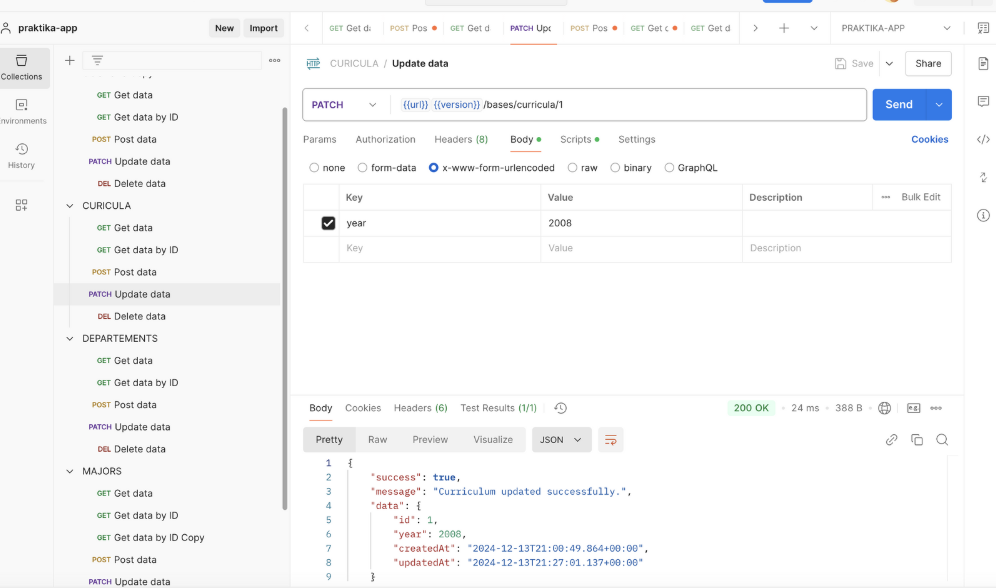
\includegraphics[width=0.9\textwidth]{gambar/postman.png}
    \caption{Pengujian API menggunakan Postman}
    \label{fig:postman_testing}
\end{figure}

Gambar di atas menunjukkan bagaimana \emph{Postman} digunakan untuk mengirim permintaan API ke server, memverifikasi respons yang diterima, dan memastikan bahwa setiap endpoint bekerja sesuai dengan yang diharapkan. Pengujian ini melibatkan berbagai skenario, seperti mengirimkan data valid, mengirimkan data yang tidak lengkap, atau menguji endpoint dengan parameter yang tidak valid.Melalui pengujian manual, otomatis, dan pengujian API menggunakan \emph{Postman}, sistem backend PraktikaApp dan PraktikaTelelab dapat dijaga kualitasnya dan dijamin berfungsi sesuai dengan spesifikasi yang telah ditentukan, serta memberikan pengalaman pengguna yang optimal.

\section{\emph{Local Development}}

Proses deployment dilakukan menggunakan Docker dan Nginx, seperti yang ditunjukkan pada gambar berikut. Pada tahap ini, \emph{port mapping} dilakukan untuk mengarahkan trafik yang datang ke domain yang sudah dikonfigurasi ke kontainer yang sesuai melalui Nginx. Misalnya, jika aplikasi frontend dan backend menggunakan port yang berbeda, Nginx akan melakukan mapping antara port pada mesin host dengan port yang digunakan oleh kontainer Docker.

Sebagai contoh, jika \texttt{service\_name.praktika.its.id.localhost} merujuk ke aplikasi frontend, maka Nginx akan mengarahkan trafik yang masuk pada port 3000 ke port yang digunakan oleh container frontend. Begitu juga dengan aplikasi backend yang dapat diakses melalui subdomain \texttt{api.service\_name.praktika.its.id.localhost}, yang akan diarahkan ke port backend di dalam kontainer Docker.Dalam hal ini, domain yang digunakan untuk mengakses aplikasi adalah \texttt{service\_name.praktika.its.id.localhost} atau \texttt{api.service\_name.praktika.its.id.localhost}, di mana \texttt{service\_name} adalah nama dari aplikasi, misalnya \texttt{praktika\_app}, \texttt{praktika\_sso}, dan \texttt{praktika\_telelab}. Setiap aplikasi ini akan memiliki kontainer-nya masing-masing, baik untuk bagian \emph{backend} (BE) maupun \emph{frontend} (FE), seperti yang ditunjukkan pada gambar di bawah \ref{deployment_diagram}.

\begin{figure}[h!]
  \centering
  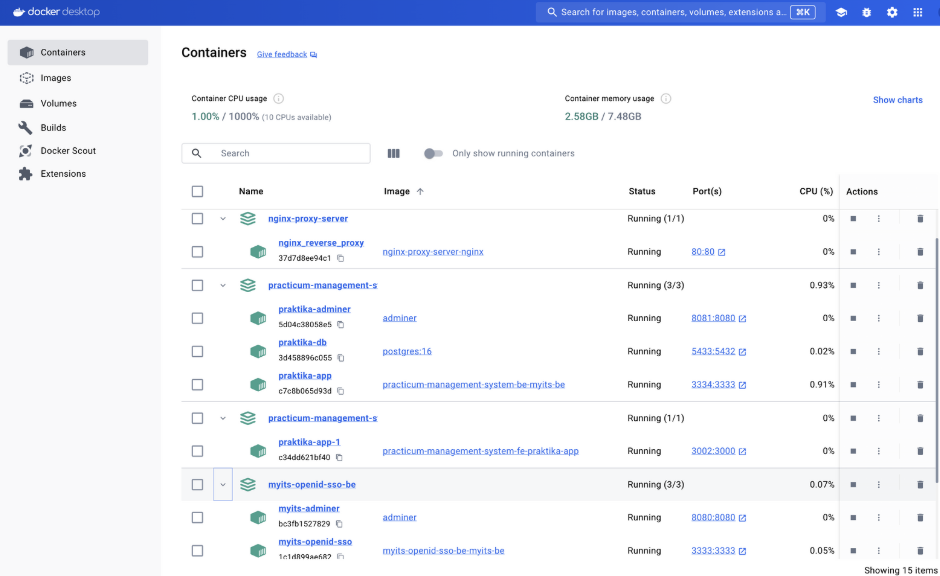
\includegraphics[width=0.7\textwidth]{gambar/docker.png}
  \caption{Diagram Deployment Sistem dengan Docker dan Nginx}
  \label{deployment_diagram}
\end{figure}

Kontainer Docker akan dibungkus dengan Kubernetes, sehingga sistem dapat dikelola dengan lebih efisien dan dapat diskalakan sesuai kebutuhan. Dengan konfigurasi ini, aplikasi akan dapat diakses di browser menggunakan domain name yang telah dikonfigurasi pada Nginx, seperti pada gambar di bawah.

\begin{figure}[h!]
    \centering
    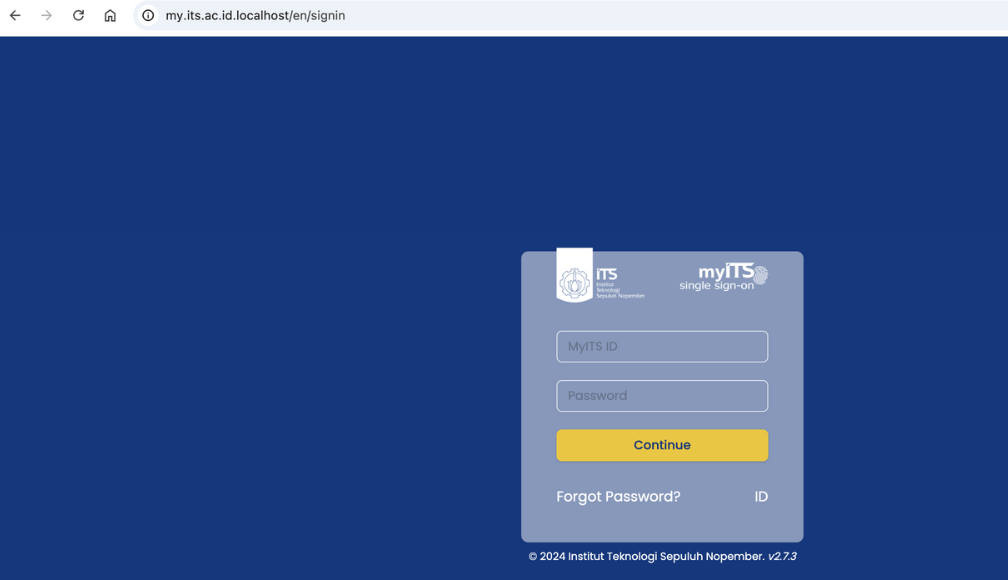
\includegraphics[width=0.7\textwidth]{gambar/sso.png}
    \caption{Aplikasi PraktikaSSO pada browser}
\end{figure}
